\documentclass[a4paper]{article}
\usepackage[spanish]{babel}
\usepackage[utf8]{inputenc}
\usepackage{charter}   % tipografia
\usepackage{graphicx}

\usepackage{subfig}
\usepackage{float}
%\usepackage{makeidx}

%\usepackage{float}
%\usepackage{amsmath, amsthm, amssymb}
%\usepackage{amsfonts}
%\usepackage{sectsty}
%\usepackage{charter}
%\usepackage{wrapfig}
\usepackage{listings}
%\lstset{language=C}


\usepackage{color} % para snipets de codigo coloreados
\usepackage{fancybox}  % para el sbox de los snipets de codigo

\definecolor{litegrey}{gray}{0.94}

% \newenvironment{sidebar}{%
% 	\begin{Sbox}\begin{minipage}{.85\textwidth}}%
% 	{\end{minipage}\end{Sbox}%
% 		\begin{center}\setlength{\fboxsep}{6pt}%
% 		\shadowbox{\TheSbox}\end{center}}
% \newenvironment{warning}{%
% 	\begin{Sbox}\begin{minipage}{.85\textwidth}\sffamily\lite\small\RaggedRight}%
% 	{\end{minipage}\end{Sbox}%
% 		\begin{center}\setlength{\fboxsep}{6pt}%
% 		\colorbox{litegrey}{\TheSbox}\end{center}}

\newenvironment{codesnippet}{%
	\begin{Sbox}\begin{minipage}{\textwidth}\sffamily\small}%
	{\end{minipage}\end{Sbox}%
		\begin{center}%
		\colorbox{litegrey}{\TheSbox}\end{center}}



\usepackage{fancyhdr}
\pagestyle{fancy}

%\renewcommand{\chaptermark}[1]{\markboth{#1}{}}
\renewcommand{\sectionmark}[1]{\markright{\thesection\ - #1}}

\fancyhf{}

\fancyhead[LO]{Sección \rightmark} % \thesection\ 
\fancyfoot[LO]{\small{Christian Cuneo}}
\fancyfoot[RO]{\thepage}
\renewcommand{\headrulewidth}{0.5pt}
\renewcommand{\footrulewidth}{0.5pt}
\setlength{\hoffset}{-0.8in}
\setlength{\textwidth}{16cm}
%\setlength{\hoffset}{-1.1cm}
%\setlength{\textwidth}{16cm}
\setlength{\headsep}{0.5cm}
\setlength{\textheight}{25cm}
\setlength{\voffset}{-0.7in}
\setlength{\headwidth}{\textwidth}
\setlength{\headheight}{13.1pt}

\renewcommand{\baselinestretch}{1.1}  % line spacing


% \setcounter{secnumdepth}{2}
\usepackage{underscore}
\usepackage{caratulaMetNum}
\usepackage{url}
\usepackage{alltt}
\usepackage{tikz}
\usetikzlibrary{matrix,decorations.pathreplacing}
\usepackage{color}
% \usepackage{gnuplottex}
\usepackage{verbatim}
\usepackage{algorithm}
\usepackage{amsmath}
\usepackage{algpseudocode}
\usepackage{listings}
\usepackage{pdfpages}
\setcounter{MaxMatrixCols}{20}
\usepackage{color}

\definecolor{dkgreen}{rgb}{0,0.6,0}
\definecolor{gray}{rgb}{0.5,0.5,0.5}
\definecolor{mauve}{rgb}{0.58,0,0.82}

\lstset{frame=tb,
  language=Python,
  aboveskip=3mm,
  belowskip=3mm,
  showstringspaces=false,
  columns=flexible,
  basicstyle={\small\ttfamily},
  keywordstyle=\color{blue},
  commentstyle=\color{dkgreen},
  stringstyle=\color{mauve},
  breaklines=true,
  breakatwhitespace=true,
  tabsize=3,
  numbers=left,
  xleftmargin=2em,
  frame=single,
  framexleftmargin=2em,
  numbersep=5pt,                   % how far the line-numbers are from the code
  numberstyle=\small\color{gray} % the style that is used for the line-numbers
 }



% ******************************************************** %
%              TEMPLATE DE INFORME ORGA2 v0.1              %
% ******************************************************** %
% ******************************************************** %
%                                                          %
% ALGUNOS PAQUETES REQUERIDOS (EN UBUNTU):                 %
% ========================================
%                                                          %
% texlive-latex-base                                       %
% texlive-latex-recommended                                %
% texlive-fonts-recommended                                %
% texlive-latex-extra?                                     %
% texlive-lang-spanish (en ubuntu 13.10)                   %
% ******************************************************** %






\begin{document}


\thispagestyle{empty}
\materia{Métodos Numéricos}
\submateria{Primer Cuatrimestre - 2015}
\titulo{Trabajo Práctico II}
\subtitulo{Reconocimiento de Dígitos: Métodos Numéricos para la clasificación de datos}
\integrante{Cuneo, Christian}{755/13}{chriscuneo93@gmail.com}

\abstracto{En este informe voy a desarrollar como solucione el problema planteado por la materia, en el cual se presentaba una base de datos, con diferentes muestras clasificadas, y al presentarse una nueva muestra, uno tenia que clasificara lo mas correctamente posible. En este caso vamos a tratar imágenes de dígitos manuscritos como datos, y el dígito que representan como la clasificación}
\palabraClave{k nearest neighbors}
\palabraClave{Análisis de componentes principales}
\palabraClave{Método de la Potencia}

\maketitle
\newpage


\vspace{3cm}
\tableofcontents
\thispagestyle{empty}

\newpage


\begin{comment}
\begin{codesnippet}
\begin{verbatim}

struct Pepe {

    ...

};

\end{verbatim}
\end{codesnippet}
\end{comment}
\setcounter{page}{1}

\section{Introducción Teórica}

La resolución de este trabajo practico tiene como cimientos dos métodos muy importantes del álgebra lineal utilizados para resolver sistemas de ecuaciones, el primero, y el mas conocido, es el método de eliminación gaussiana; el segundo es el de la Factorizacion LU

\subsection{K nearest neighbors}
El método kNN (k vecinos mas cercanos en ingles) es un un método de clasificación de datos, en este metodo ves a cada muestra, de $n$ atributos, como un elemento en el espacio $\Re^n$. Se tienen un conjunto de muestras ya clasificadas, llamado grupo de entrenamiento, y, para clasificar una muestra nueva uno calcula la distancia euclidiana:
$d(x, y)=\sqrt{\sum_{i=1}^{n}(x_i - y_i)^2}$ 
con cada muestra del grupo de entrenamiento. Luego uno almacena la clasificación de los $k$ elementos mas cercanos y asigna a la muestra desconocida la clasificación predominante del grupo de los mas cercanos.

\subsection{Análisis de Componentes Principales}

El análisis de componentes principales (PCA en español) tiene este objetivo: dadas $n$ observaciones de $p$ variables, se analiza si es posible representar adecuadamente esta información con un número menor de variables construidas como combinaciones lineales de las originales. 
% PCA construye una transformación lineal que escoge un nuevo sistema de coordenadas para el conjunto original de datos en el cual la varianza de mayor tamaño del conjunto de datos es capturada en el primer eje (llamado el Primer Componente Principal), la segunda varianza más grande es el segundo eje, y así sucesivamente. Para construir esta transformación lineal debe construirse primero la matriz de covarianza. Debido a la simetría de esta matriz existe una base completa de vectores propios de la misma. La transformación que lleva de las antiguas coordenadas a las coordenadas de la nueva base es precisamente la transformación lineal necesaria para reducir la dimensionalidad de datos. Además las coordenadas en la nueva base dan la composición en factores subyacentes de los datos iniciales.

El procedimiento utiliza una transformación ortogonal para convertir un conjunto de muestras con variables posiblemente correlacionadas, en un conjunto de muestras con variables no correlacionadas (no dependientes entre si), a estas variables las llamamos componentes principales (la cantidad de estos componentes siempre es menor o igual a la cantidad de variables originales).
Esta tranformación esta definida de una forma que el primer componente principal sea el provoque mayor variabilidad en los datos, quiere decir el de mayor varianza, el segundo sea el siguiente mayor, y así sucesivamente.


\newpage 

\section{Desarrollo}
En el presente informe se presenta la implementación, desarrollo y análisis de resultados usados en la resolución de un problema práctico, con algunas herramientas estudiadas y provistas por la materia, algunos conceptos vistos en probabilidad y estadística, y por ultimo conceptos aprendidos a medida que se iba avanzando con el trabajo. El problema principal planteado consiste en lograr reconocer una imagen de un dígito manuscrito, quiere decir, poder predecir a que dígito corresponde una imagen dada.\par
Para resolver este problema se te presenta una base de datos imágenes de dígitos manuscritos que ya se saben a que dígito corresponde cada una (grupo de imágenes "train"), y por supuesto un grupo de imágenes a las que deberás asignar un dígito utilizando alguna forma de reconocimiento (grupo de imágenes "test"). Para hacer el proceso mas simple todas las imágenes son cuadradas de 28x28 pixeles y en escala de grises.\smallbreak\par
El problema se aborda desde dos puntos de vista, el probabilista y el del álgebra lineal. El álgebra lineal se utiliza para llegar a las soluciones, y la probabilidad se utiliza para hacer este proceso de una forma mas eficiente y rendidora.\smallbreak\par
A través de la generalización uno puede ver a una imagen como una coordenada en un espacio $\mathbf{R}^{n}$, siendo $n$ la cantidad de pixeles de la imagen (en este caso 784), y como cada imagen de la base de datos de imágenes conocidas (train) es entonces una coordenada con un una clasificación conocida (su dígito); luego, una aproximación a la solución valida seria, dada una imagen desconocida, buscar que puntos mas cercanos tiene en el espacio $\mathbf{R}^{784}$, y asignarle un resultado acorde.
Ya existe un método que realiza estos pasos, y se llama K-vecinos más cercanos (Knn por su ingles "K nearest neighbors") y consiste en buscar, utilizando la distancia euclidiana, los K puntos mas cercanos a cierto punto, en nuestro caso, la imagen desconocida.\par
Luego de tener estos K puntos cercanos, uno puede clasificar a que grupo pertenece la imagen desconocida de distintas formas, en nuestro caso se utiliza la votación, básicamente teniendo estos K vecinos, buscamos al grupo dominante (la clasificación que mas veces aparece) y asignamos esta clasificación a nuestra imagen desconocida.\smallbreak\par
Al trabajar en $\mathbf{R}^{784}$ este proceso se vuelve muy lento, ya que este método se ve afectado directamente por la dimensión de los puntos que procesa, específicamente al calcular la distancia euclidiana, por esto lo que se va a buscar es reducir la dimensión de los puntos, tratando de perder la menor cantidad de características posibles de las imágenes. Otro problema es que este método se ve tocado por la maldición de la dimensionalidad, que en este caso afecta al momento de decidir que puntos son los mas cercanos al punto a clasificar, ya que si la dimensión de las muestras es muy grande, la mayoría de los vectores van a ser equidistantes, por lo tanto no se puede confiar en los resultados de la 'votacion'.\par
Es por esto que vamos a buscar alguna forma de reducir la dimensión de los datos a procesar. Aquí es donde entra en juego la probabilidad y estadística.\smallbreak\par
Vamos a buscar que pixeles de las imágenes son mas importantes y descartar los menos importantes, haciendo un análisis de componentes principales reduciendo así la dimensión en la que trabajamos. Para esto vamos a acudir al termino de la covarianza, que, aplicada a dos variables, muestra la tendencia de estas dos variables a variar juntas. Esto, aplicado a estas imágenes, vamos a buscar que puntos de las imágenes son los que mas varían entre todas las imágenes de train, obteniendo así información para saber que características (pixeles) de las imágenes son las mas importantes a analizar, las que relacionan o distinguen a una imagen de otra. Para esto vamos a calcular una matriz de covarianzas de los datos de train, ahi veremos la covarianza que tiene cada pixel con los demás pixeles de las muestras (hay que tener en cuenta que esta matriz sera simetrica, ya que la covarianza entre las variables $a$ y $b$ es igual a la covarianza entre $b$ y $a$, por definición). Lógicamente esta matriz va a pertenecer a $\mathbf{R}^{784x784}$. Para calcular esta matriz primero generaremos la matriz $X$ con una muestra de train por fila y haciendo calculos para que la media de estas sea cero, de esta forma:
$$x^{(i)} = (x^{(i)}-\mu)/\sqrt{n-1}$$
Donde $x^{(i)}$ es la fila $i$ de $X$ y $\mu$ es un vector con la media de cada variable de las muestras y $n$ es la cantidad de muestras. Luego la matriz de covarianzas $M_X$ sera:
$$M_X = X^tX$$
Como resultado $M_X$ sera:
$$M_{X (j,k)} = \frac{1}{n-1}\sum_{i=1}^{n} (x_j^{(i)} - \mu_j)(x_k^{(i)} - \mu_k)$$
Como se ve, esta es la covarianza entre la variable $j$ y $k$, y, en el caso $j = k$ el producto sera entre dos multiplicandos iguales, que serán la desviación estándar de la variable, y la desviación estándar de una variable al cuadrado es la varianza de esta.
El siguiente paso sera encontrar los autovalores mas grandes de esta matriz y sus autovectores asociados, para lograr esto se utilizara el Método de la Potencia tantas veces como autovalores se quieran encontrar. Ya teniendo estos autovectores (que tienen a los mas grandes autovalores asociados), uno puede formar una base de autovectores para poder realizar una transformación característica aplicando un cambio de base y logrando un cambio de coordenadas de las muestras, de esta forma lograremos expresar las muestras de una forma que los datos principales de la muestra original se encuentren en cada coordenada de la muestra transformada. La base de autovectores de $M_x$ sera:
$$V = (v_1,v_2,\dots,v_\alpha)$$
Siendo $\alpha$ la cantidad de autovalores y autovectores buscados (la cantidad de componentes principales). Y la transformación característica sobre una muestra $x$ se aplicara de esta forma:
$$tc(x) = V^tx = (v_1^tx,v_2^tx,\dots,v_\alpha^tx)$$
Este transformación característica se aplicará a cada muestra de la base 'train', logrando, como vimos antes, tener en cuenta solo la información mas importante y disminuyendo la dimensión de las muestras. Esta misma transformación se aplicara luego a la muestra a clasificar, y ahora, al buscar los k vecinos mas cercanos, se tardara menos en calcular las distancias euclidianas (por la reducción de dimensión) y ademas se sabrá que la clasificación sera mas acertada (por el descarte de información innecesaria y redundante).\smallbreak

\subsection{Implementación}

\subsection{Experimentación}
Los objetivos principales de la experimentación en este trabajo es averiguar cual es la mejor forma de usar las técnicas implementadas para tener las mayores posibilidades de aciertos a la hora de clasificar datos desconocidos.\newline
Para poder medir la efectividad de cualquiera de las técnicas de implementación implementadas uno tiene que aplicar los métodos para tratar de clasificar datos ya conocidos, en este punto entra en juego el concepto de Cross-Validation. Este método se basa en particionar la base de training que usamos en dos partes, una para usar de training, y otra de la cual tomaremos cada muestra y usaremos la implementación para clasificarla, para luego comparar la clasificación dada por el programa con la clasificación original de la muestra.\newline
Cross-Validation plantea realizar este procedimiento para diferentes particiones de la base de training original y analizar cual es el porcentaje de acierto de la técnica (con sus respectivos parámetros), y usando estos datos, elegir cual es la mejor técnica a utilizar, y con que parámetros, balanceando el tiempo de ejecución y con el porcentaje de aciertos.\par\smallbreak
Para mis experimentos use dos juegos de Cross-Validation, uno en el que particiono la base de training en un 10\% para usar de base de test y un 90\% para usar de base de train; y otro en el que particiono en un 20\% para la base de test y un 80\% para la base de train. Para el primer juego hice 10 particiones distintas y para el segundo 5, todas generadas aleatoriamente utilizando python, usando $int(random.uniform(1,42000))$ para generar 4200 números en el primer juego, y 8400 en el segundo (diferentes) para seleccionar las muestras para la partición de test, y el resto quedaba para usar de train.

\subsubsection{Experimentación 1: kNN}
Aquí vamos a analizar cual es el rendimiento temporal y la eficiencia del modelo de clasificación kNN. Para esto realicé un análisis utilizando Cross-Validation y midiendo los resultados variando el único parámetro de esta implementación: cuantos elementos cercanos elegir para luego hacer la votación, es decir, el $k$ de kNN.\par\smallbreak
La hipótesis principal es que el tiempo no va a variar por la cantidad de elementos que tome para hacer la votación, ya que simplemente para ver que elementos de la base de training están mas cerca de la muestra a clasificar implica medir la distancia euclidiana de cada elemento con la muestra, y este proceso es el que lleva mas tiempo, ya que luego la distancia se guardara en una cola de prioridad, y luego, la cantidad $k$ de elementos cercanos que vamos a utilizar se van a 'popear' de esta cola, que es un proceso que tarda un tiempo insignificante, ya que lo que mas tarda es 'pushearlos'. En resumen, la diferencia de tiempo entre elegir un $k$ y otro se vera en la cantidad de 'pops' a hacer para la votación, el cual es insignificante comparado con el calculo de las distancias euclidianas, que es de orden $O(n^2)$.\par
Los $k$ que tome de parámetro para pruebas los pensé luego de contar cuantas muestras de cada dígito hay en la base de training, de estas cuentas tome la mínima, y utilice la regla de tres simple para ver, si hay $x$ dígitos iguales en la base de training original, cuantos hay en la partición de training del cross-validation. Teniendo este numero uno piensa que, si usa un $k$ mayor a este numero, es seguro que se van a tener en cuenta elementos distintos al elemento a clasificar, sea cual sea.
A continuación se encontraran los resultados en gráficos, de estos experimentos. Hay que tener en cuenta que la cantidad de aciertos se calcula promediando los aciertos de cada $folding$ de cross-validation:

\subsubsection{Experimentación 2: kNN + PCA}
Esta experimentación va a analizar el rendimiento temporal y la eficiencia del modelo PCA junto al posterior uso de kNN. Para este experimento utilice como previamente dicho la técnica de Cross-Validation para analizar datos confiables, disminuyendo la probabilidad de que la elección de muestras para la base de train y la base de test afecten el resultado.\par
En este caso lo que hice fue usar la implementación de PCA + kNN variando $k$ de 0 a 1000 (ya que previamente vimos que no cuesta nada mas, temporalmente hablando) y $\alpha$ de 1 a 60 (30 a 60 para el segundo juego de Cross-Validation, por cuestiones de tiempo); y luego para cada instancia:
\begin{itemize}
\item Medir el tiempo de ejecución del cambio de base al grupo de muestras de train, utilizando la transformación ortogonal obtenida gracias al análisis de componentes principales.
\item Medir el tiempo de ejecución del procedimiento de kNN con el nuevo set de train de menores dimensiones.
\item Medir la eficiencia de la técnica y sus parámetros checkeando cuantas calificaciones correctas acertó.
\end{itemize}\par
Como uno esta haciendo un análisis de componentes principales, al variar $\alpha$ uno decide cuantos componentes principales va a tener en cuenta para hacer la reducción de dimensiones, siempre empezando por el componente principal que abarca la información mas importante de los datos, hacia la que abarca detalles que no van a servir al tratar de distinguir un dato de otro. Sabiendo esto, uno espera que, al ir aumentando el $\alpha$, el hit rate del método vaya aumentando mientras se esté considerando nueva información relevante, y, una vez que se llegue a abarcar toda la información relevante, aumentar el $\alpha$ no hará mas que considerar datos irrelevantes o demasiado detallistas, entonces el hit rate se estabilizara; si uno sigue aumentando el $\alpha$, uno supondría que, al estar tomando en cuenta mas información irrelevante que relevante, el hit rate se vera disminuido.\par
Teniendo en cuenta esto, me pareció lógico aplicar el método para distintos $\alpha$ hasta que el hit rate se estabilice, y ahí sabremos (no con 100\% certeza) que hemos llegado al punto en el que la eficiencia dejara de seguir aumentando positivamente.\par\smallbreak
Decidí no medir el tiempo de computo que requiere generar la matriz de covarianzas, ya que esta depende unicamente del tamaño de la base de train, que es fija para cada Cross-Validation distinto, por lo tanto no me parecía un dato interesante.
\smallbreak
Veamos los resultados de esta experimentación:

Para estos gráficos promedie los hit-rates de todas las particiones de cada juego de Cross-Validation por separado
Ahora veremos cual fue el promedio de todos los hits-rates para cada alpha:
\smallbreak
Y por ultimo los tiempos de cambio de base de la base de train, y del que tarda kNN en decidir la clasificación:
\smallbreak
\par
De estos resultados se pueden sacar las siguientes conclusiones:
\begin{itemize}
\item El tiempo de computo del cambio de base aumenta linealmente a medida que aumenta el $\alpha$, esto sucede porque va a haber que multiplicar cada muestra de la base de train por un autevector mas, para agregar una dimensión mas a la muestra a usar luego. El tiempo que lleva hacer el producto entre la muestra y el autovector va a ser siempre el mismo, ya que es el producto entre un vector de 784 con otro de 784, por lo tanto tomara tan solo 784*784 operaciones en todos los casos, si este tiempo también se viera afectado por el cambio de $\alpha$, entonces estaríamos hablando de un orden de computo $O(n^2)$ pero como no es así, el orden de complejidad temporal es de $O(n)$ como muestran los resultados de tiempo. Ademas como se ve, el resultado es prácticamente igual en para ambos juegos de Cross-Validation.
\item El tiempo de computo de kNN también aumenta linealmente a medida que aumenta el $\alpha$, esto es porque el procedimiento de calculo de distancias se va a hacer entre la muestra y la misma cantidad de muestras de train anterior, lo único que cambia es que cada muestra de train, al igual que la muestra desconocida, al aplicarles el cambio de base tendrán una dimensión mas que en el caso interior, esto hará que calcular las distancias euclidianas cueste una iteración mas, al verse afectado solo ese tiempo de computo, el orden de complejidad temporal sera de $O(n)$. En este caso también los resultados fueron consistentes entre los dos juegos de Cross-Validation.
\item La efectividad del método de clasificación al variar $\alpha$ se vio afectada de una forma mas fuerte desde el $\alpha = 1$, en el cual la efectividad era muy baja, al $\alpha = 10$ donde se empieza a estabilizar, luego sigue subiendo mas lentamente hasta llegar al $\alpha = 18$, donde se estabiliza casi pareciendo constante. Desde este $\alpha$ la tasa de aciertos va aumentando muy levemente hasta encontrar su pico máximo en $\alpha = 39$ para el primer juego de CV y en $\alpha = 36$ para el segundo, luego de estos valores, la tasa de efectividad baja muy levemente y se queda oscilando, pero no logra superar el pico anterior, al menos en este rango de $\alpha$. Al llegar al pico, el hit-rate es del 97,54\% y del 97,40\% para cada CV respectivamente. Lo que hay que destacar es que desde el $\alpha = 20$ aproximadamente ya se esta dentro del 97\% de efectividad, entonces se ve que el método es bastante efectivo desde un $\alpha$ bastante mas chico, esto va a ser útil a la hora de balancear entre efectividad y tiempo de computo.
\item La efectividad del método al variar $k$ es notable, se ve por los resultados que el mejor $k$ a utilizar es el $k = 3$. Es muy interesante ver que, con $k = 1$ el método ya es bastante efectivo, pero al elegir $k = 2$ la efectividad se ve reducida notoriamente, esto tiene que ser ya que, al hacer la votación uno mide el máximo en cantidades de 'votos', y al haber solo dos, va a, o haber dos votos del mismo, en ese caso se elige ese, o haber uno para una clasificación y otro para otra clasificación, y en este caso, al estar uno tomando un simple máximo, va a elegirse el primero que se llegue con la iteración del algoritmo de 'máximo', entonces va a haber una probabilidad del 50\% de elegir la clasificación correcta. Luego al elegir $k = 3$ siempre va a haber un desempate, al menos que sean tres votos diferentes, que seria de esperar que fuera un caso raro.
\end{itemize}
\section{Conclusiones}


\section{Referencias}
Los conceptos los tome de:
\begin{itemize}
\item Las clases teóricas y practicas de la cátedra.
\item Matrix Computations - Gene H. Golub, Charles F. Van Loan - JHU Press, Oct 15, 1996
\item Numerical analysis - Richard L. Burden J. Douglas Faires - 2011
\end{itemize}
\section{Apéndice: A}
\begin{center}
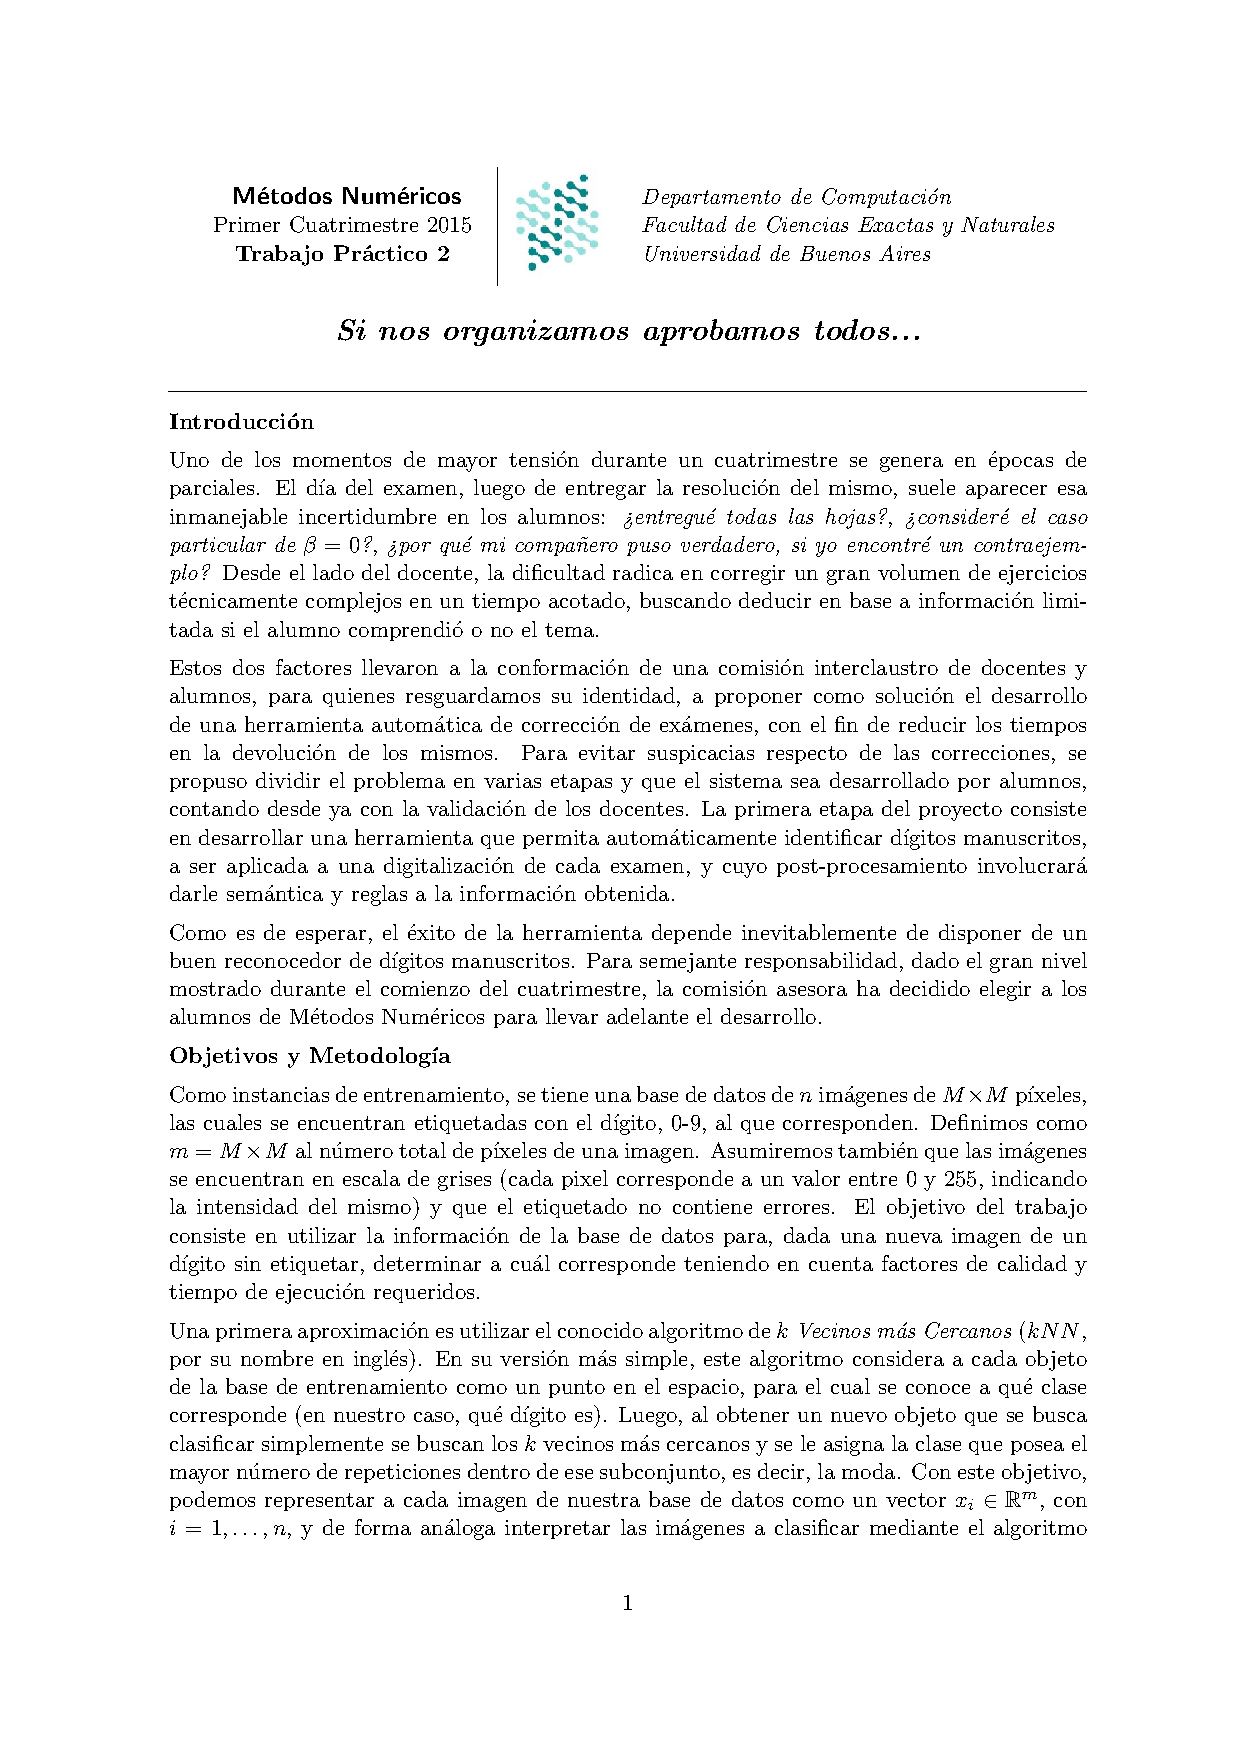
\includepdf[pages={1, 2, 3, 4}]{tp2.pdf}

\end{center}
\newpage
\section{Apéndice: B}

Scripts Experimentos:
\begin{lstlisting}
  for x in range(0,PRECISION+1):
    outp = subprocess.check_output([ bindir +"tp", param1, param2, param3, param4]).split(',')
    if (len(outp) < 3): continue
    microseconds = int(outp[0])
    if (microseconds != 0):
        time.append(microseconds)
  done += 1
  print("G="+ param4 + "  Set=" + test + "  Method=" + param3 + ' | ' + str(done) + "of" + str(total) + " | Process " + "{0:.2f}".format(float(done*100)/float(total)) + "%" + " | " + str(outp))
  ou.write(test + ',' + str(method) + ',' + str(granul) + ',' + str(int(trimmean(sorted(time), 0.25))) + ',' + outp[1] + ',' + outp[2] + "\n")
ou.close()
\end{lstlisting}

\end{document}

